
% Many thanks to Andrew West for writing most of this file
% Main LaTeX file for CIS400/401 Project Proposal Specification
%
% Once built and in PDF form this document outlines the format of a
% project proposal. However, in raw (.tex) form, we also try to
% comment on some basic LaTeX technique. This is not intended to be a
% LaTeX tutorial, instead just (1) a use-case thereof, and (2) a
% template for your own writing.

% Ordinarily we'd begin by specifying some broad document properties
% like font-size, page-size, margins, etc. -- We have done this (and
% much more) for you by creating a 'style file', which the
% 'documentclass' command references.
\documentclass{sig-alternate}
 
% These 'usepackage' commands are a way of importing additional LaTeX
% styles and formattings that aren't part of the 'standard library'
\usepackage{mdwlist}
\usepackage{url}

\begin{document} 

% We setup the parameters to our title header before 'making' it. Note
% that your proposals should have actual titles, not the generic one
% we have here.
\title{CodeScore}
\subtitle{Dept. of CIS - Senior Design 2013-2014\thanks{Advisor: Chris Murphy (cdmurphy@cis.upenn.edu).}}
\numberofauthors{4}

\author{
Allison Pearce \\ \email{alpearce@upenn.edu} \\ Univ. of Penn \\ Philadelphia, PA
\and Spencer Lee \\ \email{lesp@upenn.edu} \\ Univ. of Penn \\ Philadelphia, PA
\and Tanvir Ahmed \\ \email{tanvir@upenn.edu} \\ Univ. of Penn \\ Philadelphia, PA
\and Will McDermid \\ \email{wmcd@upenn.edu} \\ Univ. of Penn \\ Philadelphia, PA}

\date{}
\maketitle

% Next we write out our abstract -- generally a two paragraph maximum,
% executive summary of the motivation and contributions of the work.
\begin{abstract}
  \textit{The technology industry lacks automated tools for evaluating software quality. These tools would be helpful for individuals desiring to improve their abilities, recruiters searching for top programmers, and educators needing to quickly assess student performance. We propose to develop an application that calculates a metric for internal quality by detecting code smells, easily recognized design weaknesses that may indicate more significant problems within the system. The program will recognize code smells using a set of specific rules. It will then use the results to compute a CodeScore: a single value that reflects the maintainability and understandability of the piece of software based on the presence of code smells. }
\end{abstract}

% Then we proceed into the body of the report itself. The effect of
% the 'section' command is obvious, but also notice 'label'. Its good
% practice to label every (sub)-section, graph, equation etc. -- this
% gives us a way to dynamically reference it later in the text via the
% 'ref' command.
\section{Introduction}
\label{sec:intro}
Software failures result in annoyed users at best, and they can cause catastrophic system failures at worst. Six people received massive radiation overdoses from a radiation therapy device in one of the canonical examples of a fatal software error \cite{leveson1995therac}. Failures are consequences of poor software quality. Software quality is defined as ``conformance to explicitly stated functional and performance requirements, explicitly documented development standards, and implicit characteristics that are expected of all professionally developed software" \cite{pressman1997}. In addition to causing failures, disregard for software quality is expensive and inefficient, requiring more dollars and man-hours to maintain, test, and add features to project than should be necessary. An increasing appreciation of well-designed software has been manifested in the international standard for software quality, ISO/IEC 25010. The standard affirms the importance of specifying and measuring characteristics of quality, and it defines quality models intended to aid in accomplishing these goals \cite{iso2011iec}.

Software quality is commonly divided into internal quality and external quality. External quality describes how well the software meets performance expectations, and encompasses characteristics such as correctness, accuracy, integrity, robustness, reliability, usability, adaptability, and efficiency. Internal quality describes how well the software was designed and implemented, and is concerned with maintainability, flexibility, portability, reusability, readability, understandability, and testability \cite{mcconnell1993codecomplete}. Internal and external quality are closely related, and deficiencies in internal quality lead to deficiencies in external quality. For example, code that is difficult to understand will also be difficult to adapt to new requirements, and code that cannot be easily tested will likely be incorrect or unreliable. 


%projects bigger -> quality more important
%costs in terms of time, efficiency, monies, man-hours

One way to diagnose internal quality issues is by detecting code smells. Code smells are easily recognized design weaknesses that may indicate deeper, more significant problems within the system. Some common code smells include:
\begin{itemize}
\item Classes or methods that have too many lines of code
\item Duplicated code
\item Long lists of parameters for functions
\item Overly complex conditional logic
\item Inconsistent or uncommunicative naming conventions
\end{itemize}

Individual code smells are directly related to problems with specific aspects of internal quality. For example, overly complex conditional logic and inconsistent naming conventions hurt understandability and readability. Duplicated code implies that changes will have to be made not once but everywhere that the duplication occurs, which hurts maintainability. 

The proposed application tests for the presence of code smells in order to evaluate internal quality. We will define rules for custom algorithms to detect code smells, and the results of the detection will be used compute an internal quality score for a code sample. The program focuses specifically on how code smells relate to two elements of internal software quality, maintainability and understandability. These elements are underemphasized in most classroom settings. Students work quickly and haphazardly to meet deadlines and never revisit their program after turning it in, so there is no need to write maintainable or understandable code.  However, understandability and maintainability are critical outside of the classroom, where teams of developers need to understand code they did not write, and to maintain it for years as the product evolves. The proposed tool will help students assess and improve these necessary software engineering skills by providing objective feedback to make them aware of their weaknesses. Computer science teachers can use the the application when grading assignments to assess quality without spending hours reading through each student's source code. It will also allow recruiters to identify potential employees who will contribute to their company's products with a high regard for quality. Overall, this tool will help the technology industry to train and recruit a strong developer workforce who will write programs that are internally sound. 

\section{Related Work}
\label{sec:related_work}
In this section, we will provide background information on the different methods of analyzing code, the standards for measuring code quality, and various services and applications that already strive to provide quantitative analyses of code quality.


\subsection{Code Analysis Methodologies}
The majority of existing applications for measuring code quality rely on well-established code analysis techniques. These techniques involve breaking code down into specific units and measuring the counts of these units. Such techniques include parsing the source code into control structures \cite{mccabe1976complexity}, tokens \cite{halstead1977elements}, assembly instructions \cite{park1992software}, or objects \cite{chidamber1994metrics}. Once the source code has been parsed into some unit (this process is called static analysis), the attributes of the code, such as reliability, security, efficiency, size, and maintainability can be measured from the parsed results. The actual approach to measuring these attributes originated in \cite{boehm1976quantitative} and later became part of the ISO/IEC 25000 series of standards relating to the quality and evaluation of software \cite{iso2011iec}. These techniques and standards comprise the foundation for today's code quality measurement applications, and they will be the basis for the proposed approach as well.

\subsection{Ohloh}
Launched in January of 2006, Ohloh \cite{allen2009ohloh} is web service and online community owned by Black Duck Software which provides basic metrics for over 650,000 open source projects containing over 24,000,000,000 lines of code located in over 620,000 source code repositories and managed by more than 3,000,000 contributors. These projects are retrieved from source control repositories and analyzed. Metrics such as lines of code, amount of source code comments, and estimated software cost (based on the COCOMO model \cite{boehm2000software}) are provided, along with commit statistics, project activity, and programming language detection. This data is graphically displayed when one views a project's information on the site. Ohloh also provides global statistics across all projects for different programming languages and contributor statistics for different authors of open source code. 

Ohloh primarily focuses on tracking project/contributor activity for large open-source projects. The proposed application will focus more on providing code quality-oriented metrics.

\subsection{Common Weakness Enumeration}
The Common Weakness Enumeration (CWE) \cite{mitre2006cwe} is a community-developed list of software weaknesses hosted by the MITRE Corporation. The CWE was developed with the intention of providing:

\begin{itemize}
\item a common standard of identifying, mitigating, and preventing software weaknesses.
\item a common source of measuring weaknesses for software security tools.
\item a common language for describing the various types of software weaknesses that exist in computer architecture, software design, and source code.
\end{itemize}

CWE supports the discovery of common types of software security flaws such as buffer overflows, handler errors, pathname traversals, and resource management errors (amongst others) within code.

CWE began with the Common Vulnerabilities and Exposures (CVE) list in 1999 \cite{mitre2005cve}. As part of the SAMATE project \cite{nist2005samate}, MITRE later expanded upon the CVE list with the Preliminary List of Vulnerability Examples for Researchers (PLOVER) \cite{christey2005plover}. PLOVER was the first attempt to take real-world examples of software vulnerabilities and abstract them into common classes of more general vulnerabilities that can arise during the software development process. The goal of PLOVER was to make this information available to developers, researchers, and analysts so that they may use it for a variety of purposes, with the goal of improving code security. CWE encompasses much of the CVE list and expands upon PLOVER by establishing community-developed definitions and descriptions of these common weaknesses.

CWE primarily strives to provide standards relating to the weaknesses of code in terms of security. This may be a valuable resource for the proposed application, as many code weaknesses are indicative of, or are themselves, code smells.

\subsection{Other Static Code Analysis Tools}
A wide variety of other static code analysis tools also exist. The Web Application Security Consortium provides a community-sourced list of some commonly used tools for code analysis \cite{webappsec2012}. Some of these tools include:

\begin{itemize}
\item CodeSonar - A full-featured code analysis tool with binary analysis, results visualization, and a wide variety of metrics. CodeSonar can detect numerous code faults and security risk within projects containing up to millions of lines of Java, C, or C++ code \cite{grammatech2013codesonar}.
\item Klocwork Insight - Provides a wide range of metrics with detailed reports and offers integration with a variety of IDEs \cite{klocwork2013insight}.
\item FindBugs - Open-source code analysis tool which is capable of detecting many different types of bugs in Java code \cite{pugh2013findbugs}.
\item Yasca - An open-source code analysis tool combining the functionality of many other open-source code analysis tools in order to provide quality and security metrics for code written in a wide range of languages \cite{scovetta2007yasca}.
\end{itemize}

The proposed solution will attempt to provide more functionality than the majority of open-source, similar applications. We aim to provide quality of functionality similar to commercial-grade applications, while making it accessible to a wider audience and not merely for large companies.

\section{Project Proposal}
\label{sec:project_proposal}
We propose to design a process that will be used to quantitatively assess code quality. A user will upload examples of his or her code to a server, where the program will evaluate its internal quality by detecting code smells. Focusing on static, internal quality allows for the quantification of source code's quality without becoming biased by different system architectures or environments. Code smells provide a useful indicator of these metrics because they are specific and detectable, and because there is existing work which can be used as a starting point \cite{moha2009duchien}, \cite{palomba}.  The scope of this project will be limited to just two important metrics of internal quality, understandability and maintainability. 
	
\emph{Understandability}, a measure of how easy a code sample is for a human to interpret, can be estimated in part by the length of message chains (a code smell in which one method invokes another, which invokes another, and so on in a long sequence of function calls), length of parameter lists, by determining what fraction of variable names are dictionary words versus strings of letters and numbers, and by analyzing the class structure of a program. 

\emph{Maintainability}, a measure of how easy a code sample will be to update and change, can be estimated in part by detecting and recognizing coupling between classes, duplicated code, and classes that are too large. Another indicative code smell is shotgun surgery, which describes the situation in which changing one behavior requires numerous changes to code in different places. For example, if logging statements are implemented separately in each function in a class, then adding line numbers to the logs will take considerable effort. A better solution would be to write a log wrapper for all of the functions, so that any changes only need to be made once. 

The proposed application will detect specific code smells that pertain to understandability and maintainability. The results of this detection will then be combined into an overall score for the code sample. The program will provide a detailed score report describing the number, type, and location of problems in the code. This report can be shared with recruiters as a quick and objective evaluation of a candidate's programming ability, used as a tool for self-improvement, or incorporated into teachers' grading rubrics. 

\subsection{Anticipated Approach}
\label{subsec:approach}

We have prioritized the code smells for which we will implement detection algorithms. The algorithms we propose will operate on Java programs. Some code smells are simpler to detect than others, and we will begin by writing detectors for the following:
\begin{itemize}
\item Long parameter lists, long methods, and large classes. The input will be parsed into tokens, and specific token patterns will be used to identify the beginnings and ends of parameter lists, methods, and classes.
\item Duplicated code.  For smaller programs, a line-by-line comparison is feasible. For larger programs, the input can be parsed into control flow blocks, and blocks can be compared for duplication. 
\item Poor naming conventions. The input will be parsed into tokens, assuming variable names are to the left of an equal sign. Names will be matched with dictionary words, and those that have no relationship to English words will detract from the understandability score. Words that are not suited for variable names, like ``something" or ``anywhere," will be blacklisted so that they will not affect the metrics aversely.  Additionally, names that contain type information will detract from the maintainability score because those names would have to be changed throughout the program in the event that the variable's type changed.
\item Message chaining. For each line of the program, a regular express can be used to identify instances of chained method calls (in Java, several periods and sets of  parentheses). 
\end{itemize}
We will next investigate more challenging code smells. Some will require more than just the source code to detect. There are maintainability issues that have been shown to be detectable using revision history from version control \cite{palomba}, and we would like to incorporate at least one of these into the analysis.  As described previously, shotgun surgery is a problem that indicates that changing one behavior requires several separate changes in the code.  This antipattern can be detected by parsing revision histories to determine if certain lines of code in different parts of the program tend to changed at the same time.

Other interesting code smells pertain to inappropriate relationships between classes. Feature envy is a problem in which methods in one class repeatedly use data and methods from another class. We can detect this code smell by first parsing all of the files in the input to determine which classes are available, and then tokenizing type information within each class to determine if there is extensive overlap. 

We will also search for overly complex conditional logic, such as deeply nested if statements and loops. This issue can be detected by searching for specific tokens, such as ``if," ``else," ``for," and ``while," and using indentation and ending brackets to assess nesting.

Of the code smells the program will detect, large classes, long methods, duplicated code, poor naming conventions, feature envy, and shotgun surgery detract from maintainability. Long parameter lists, long methods, large classes, poor naming conventions,complex conditional logic, and message chaining detract from understandability. A maintainability score and an understandability score will be computed using the results of the relevant code smell detection algorithms. The scores will be informed by the frequency and severity of the issues (one poorly named variable is less problematic than five duplicated code blocks), and the sum of these two scores will be reported as the overall CodeScore.

It is possible that not all of these code smells will provide unique information. Some code smells might be so correlated with others that performing the additional detection is not worth the increased processing time. If this is the case, we will discard one of the correlated smells and replace it with a more informative metric.

Processing will be performed from a code repository on an Amazon Web Services (AWS) EC2 machine. EC2 is a service that provides resizable computing capacity in the cloud. A user can upload their code to this endpoint, where it will trigger the application. On the EC2 machine, a controller class will coordinate a pool of worker threads. When software is uploaded to the endpoint, the controller class will generate $n$ workers, where $n$ is the number of detection algorithms to be performed on software sample. Then each of the workers will perform the detection tasks as described previously. Once complete, the controller will then reduce all of the data computed by the workers and summarize the findings. The workflow for the system is shown in Figure 1. 

One drawback of this method is that it is largely centralized. If the server containing the controller code is compromised at any time during the computation, all progress in the analysis will be lost. A reach goal or future development is to decentralize the process so that loss of a server does not result in complete loss of progress. Ideally, this could be implemented using MapReduce \cite{dean2008mapreduce}.


\begin{figure}[htb!]
	\begin{center}
		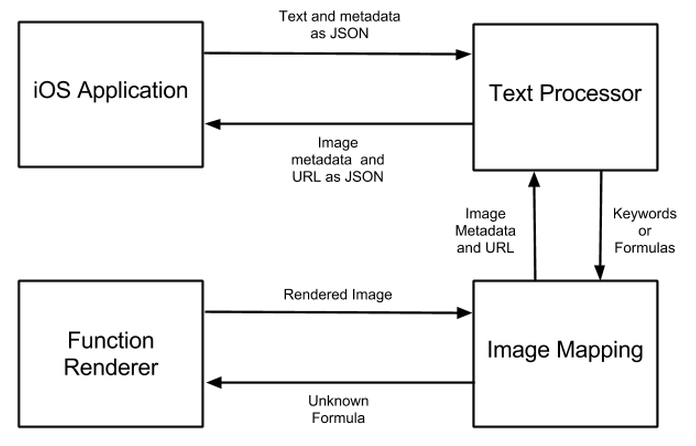
\includegraphics[width=0.9\linewidth]{block_diagram}
	\end{center}
	\vspace{-12pt}
	\caption{Block diagram of the system}
	\label{fig:some_graph}
\end{figure}

\subsection{Technical Challenges}
\label{subsec:tech_challenges}
Though we have described the rules we plan to apply to detecting each type of code smell, fine-tuning the detection algorithms to meet the evaluation criteria will be difficult. Each code smell will pose unique challenges, especially those involving analysis of multiple classes or complex parsing. We will conduct a series of experiments to evaluate the performance of the algorithms and to determine the optimal parameters, such as patterns to search for. In many cases, we will not have an existing detector to compare results with, but this can be overcome by comparing with human detection. 

Another challenge is developing the model for combining the results of individual code smell detections into a comprehensive assessment of maintainability and understandability. One novel goal of this project is that it aims to provide a holistic assessment of internal software quality that can be computed quickly, in contrast with most similar programs which search for a single specific defect. We will need to perform additional experiments to determine the proper weights for each code smell in the overall scoring model, and to compare these results with human judgement.

Parsing source code effectively and efficiently poses a third challenge. This task is crucial to the project, because we need to analyze code at the character, token, block, and class levels. There are obvious brute-force approaches, but evaluating large software projects will require an elegant way to calculate all of the metrics in a time and space efficient manner. The shotgun surgery detection involving the version control history will be particularly interesting. Most version control systems offer change logs with a file-level granularity, but shotgun surgery requires analysis of methods within a class. This does not mean that the needed method-level granularity cannot be determined from a version control log; it only means that it is not advertised as such, and more effort will be needed to parse it. 

One advantage of this project is that if the challenges prove to be more difficult that we expect, we can remove certain code smells from consideration; similarly, if it is easier than we expect, we can define additional metrics for analyzing software quality and add them to the model.

\subsection{Evaluation Criteria}
\label{subsec:eval_criteria}

Since the project aims to quantitatively analyze code quality to, the evaluation criteria will revolve around checking how accurate the algorithm is in detecting this. We aim to test:

\begin{itemize}
\item How accurately we detect code smells.
\item How accurate the analysis is when compared to human analysis.
\end{itemize}

We hope that by measuring across these three areas, we will be able to validate that the application works as expected. As a goal for the project, we hope to hit 75\% accuracy rates on the first two criteria and hope to beat human analysis at least 50\% of the time.

For the detection of code smells, we can use precision (fraction of detected problems that are really problems) and recall (fraction of problems that are detected) to evaluate the performance. The goal will be to achieve at least 90\% for both precision and recall with each code smell detector. To do this test systematically, we will feed code through the application that has a fixed number of code smells. For example, we feed in a piece of software that has a total of 10 code smells and check how many code smells the algorithm detects. We have to test for false positives and false negatives. In both these cases, it will imply that the algorithm is not accurate as it should be. We hope that the application will have a < 10\% rate for false results. 

The second variant of testing that we can do is human testing. We can give small software packages, comprising of 10 source files each, to the application and real developers. The application will compute the CodeScore as well as all of the other metrics about the code. Real developers will then use their best judgement to analyze the code and assign each of the project's CodeScores based on how they found code smells and how they impacted code quality. The goal is to get to a point where the discrepancy between the CodeScores generated by the application and the real developers happens only 25\% of the time or less. To phrase it differently, we hope that at least 75\% of the time, there will be a rough match between the computed CodeScores. (Rough match is determined by +/- 10\%)

\section{Research Timeline}
\label{sec:research_timeline}
\begin{itemize*}
	\item {\sc already completed}: Performed research on measuring internal code quality. Began looking into parsing techniques for source code and detecting code smells.\vspace{3pt}
	\item {\sc prior to thanksgiving} : Have a basic worker class and controller running. The controller should be able to spawn off workers when the server-side repository is updated.\vspace{3pt}
	\item {\sc prior to christmas} : Have worker class implemented. Should be able to detect at least three code smells and report back to controller. Controller should be able to reduce the output.\vspace{3pt}
\item {\sc by the start of spring term} : Implement at least three more detection algorithms.\vspace{3pt}	
\item {\sc by the end of march} : Implement remaining detection algorithms (time permitting). Test performance and fine-tune previously implemented algorithms. \vspace{3pt}
\item {\sc reach goals} : Investigate how to change design to map reduce. Look for more code metrics to measure and incorporate. Add additional code smells. \vspace{3pt}
\item {\sc completion tasks} : Verify implementation meets requirements. Conduct testing mentioned in evaluation section. Complete write-up.\vspace{3pt}
\end{itemize*}

% We next move onto the bibliography.
\bibliographystyle{plain} % Please do not change the bib-style
\bibliography{prop_spec}  % Just the *.BIB filename

% Here is a dirty hack. We insert so much vertical space that the
% appendices, which want to begin in the left colunm underneath
% "references", are pushed over to the right-hand column. If we looked
% hard enough, there is probably a command to do exactly this (and
% wouldn't need tweaked after edits).
\vspace{175pt}

% We then use appendices to share some additional information with
% you, though you won't need appendices in your own proposal.

% The usage of 'enumerate' (similar to 'itemize') we talked about
% above

% You may also notice we have many 'vspace' commands lying
% around. These create 'vertical space' and are a way to force LaTeX
% to cooperate, sometimes. Don't get too involved with using them
% initially, though, because adding or deleting a single line of task
% can dramatically change how LaTeX chooses to format, page, and space
% the document
\end{document} 

